\pdfoutput=1
\documentclass[11pt]{article}
\usepackage{acl2023}
\usepackage{times}
\usepackage{latexsym}
\usepackage[T1]{fontenc}
\usepackage[utf8]{inputenc}
\usepackage{microtype}
\usepackage{inconsolata}
\usepackage{graphicx}
\usepackage{booktabs}
\usepackage{amsmath}
\raggedbottom

\title{Meaning-Preserving Paraphrase Robustness: Evaluating Lexical, Embedding, and LLM-Based Similarity Methods Under Graded Paraphrasing}

\author{Priya Gawshinde \And Jasvindar Singh \And Jaismeen Kaur \\
  DA6024 Course Project}

\begin{document}
\maketitle

\begin{abstract}
Can a computer tell that two sentences mean the same when the words change? We rewrote 300 sentences at five paraphrase levels, removed rewrites that changed the meaning, and tested TF-IDF, BM25, SBERT, two trained classifiers and an LLM judge. Every local method held up while rewrites kept most of the words, then fell sharply on the heaviest rewrite (word overlap .15): TF-IDF dropped to .502 accuracy and SBERT to .676. SBERT degraded less, and its AUC of .967 shows that much of its loss came from a fixed cutoff, not the embeddings. On the adversarial PAWS test, every local method scored below the .558 gained by always answering “different”, although SBERT's AUC of .63 shows some signal. The LLM judge scored .988 at the heaviest level and .842 on 500 PAWS pairs where SBERT scored .502, but took about 150 times as long per pair and was limited by a daily quota.
\end{abstract}

\section{Introduction}
Duplicate-question detection, plagiarism checks and search all need to decide whether two pieces of text say the same thing. A person can do this even when almost every word changes. A method that only counts shared words cannot, while a method that looks at meaning may still miss small changes that flip a sentence, such as swapping who did what. These two failure modes pull in opposite directions: a method tuned to accept heavy rewording will also tend to accept a sentence whose roles have been swapped, and a method that insists on shared words will reject honest paraphrases.

Most benchmarks report one accuracy number per dataset, which hides where a method starts to fail. This project instead measures how each kind of method copes as rewriting gets heavier, by building a ladder of paraphrases from light synonym swaps to aggressive rewrites, and tests the opposite case with adversarial pairs that keep the words but change the meaning. It also measures what the better methods cost to run. We asked three research questions:
\begin{itemize}\setlength{\itemsep}{1pt}\setlength{\parskip}{0pt}
\item \textbf{RQ1.} Does SBERT degrade more gracefully than TF-IDF and BM25 as paraphrasing gets heavier?
\item \textbf{RQ2.} At what paraphrase level does each method fall below a usable threshold?
\item \textbf{RQ3.} Does an LLM judge beat trained classifiers on hard adversarial cases, and at what cost?
\end{itemize}
Our contributions are:
\begin{itemize}\setlength{\itemsep}{1pt}\setlength{\parskip}{0pt}
\item a five-level paraphrase ladder of 2,202 labelled pairs built from 300 sentences, with a meaning check and a measured word overlap for every level;
\item a comparison of six methods on the ladder, on PAWS, MRPC and QQP, and on time and money cost;
\item an analysis showing that much of the heavy-rewrite failure comes from where the yes/no cutoff sits, and that word overlap explains failure better than the level number;
\item a human check of the LLM-made labels, reported both blind and after review.
\end{itemize}

\section{Related Work}
\textbf{Lexical similarity.} TF-IDF \citep{salton1988} weights each word by how rare it is across a collection and compares sentences as weighted word vectors. BM25 \citep{robertson2009} adds term-frequency saturation and length normalisation and is a standard baseline in retrieval. Both only see words that the two texts share.

\textbf{Sentence embeddings.} Sentence-BERT \citep{reimers2019} fine-tunes BERT in a Siamese set-up so that a whole sentence maps to one vector, and cosine similarity between vectors measures meaning. Two sentences can be close without sharing any words.

\textbf{Paraphrase data.} MRPC \citep{dolan2005} contains news sentence pairs labelled as paraphrases or not. QQP, distributed with GLUE \citep{wang2018}, contains Quora question pairs labelled as duplicates. PAWS \citep{zhang2019} was built to expose models that rely on word overlap: its pairs are made by swapping words and back-translating, so many share almost all their words while differing in meaning. \citet{zhang2019} showed that strong models trained without such pairs do poorly on them.

\textbf{Generating paraphrases.} Back-translation through another language is a long-standing way to produce paraphrases \citep{mallinson2017}; we use the OPUS-MT models \citep{tiedemann2020}. WordNet \citep{miller1995} supplies synonyms for light rewrites.

\textbf{LLMs as judges.} Large language models are increasingly used to grade text, with good agreement with people on many tasks \citep{zheng2023}, but they can favour text they generated themselves \citep{panickssery2024}. This is why our paraphrases and our judge come from different model families.

\section{Data}
\textbf{Base sentences.} We used 300 sentences: 150 SQuAD questions \citep{rajpurkar2016} and 150 AG News statements \citep{zhang2015}, 8 to 25 words long and chosen with a fixed random seed (42). Mixing questions and statements avoids testing only one sentence type. Neither source is in the classifier training data. Every sentence had to allow at least two WordNet word swaps, so that Level 1 changes something real. For AG News we used only the second and later sentences of each article, because the first is joined to the headline.

\textbf{Labelled datasets.} Table~\ref{tab:data} lists the labelled datasets. QQP's test labels are hidden, so we split its validation set into 5,000 pairs for tuning and 35,430 held out for testing.

\begin{table}[t]
\centering\small
\begin{tabular}{@{}lrrr@{}}
\toprule
\textbf{Dataset} & \textbf{Train} & \textbf{Validation} & \textbf{Test} \\
\midrule
PAWS & 49,401 & 8,000 & 8,000 \\
QQP & 363,846 & 5,000 & 35,430 \\
MRPC & 3,668 & 408 & 1,725 \\
\bottomrule
\end{tabular}
\caption{Labelled pairs per split. The classifiers were trained on all PAWS and MRPC training pairs plus 50,000 sampled QQP pairs, 103,069 in total.}
\label{tab:data}
\end{table}

\section{Method}
\subsection{Paraphrase levels}
Each level was made directly from the original sentence, so errors do not build up across levels (Table~\ref{tab:levels}). Level 1 replaces two or three nouns, verbs or adjectives with the most common WordNet synonym, skipping names, numbers and question words. Levels 2 to 4 used Qwen (\texttt{qwen3.8-27b}, through Groq) with three prompts: change only the grammatical structure, rewrite minimally, and rewrite aggressively (Appendix~\ref{app:prompts}). Level 5 translated each sentence into Chinese and back with MarianMT. We tried three other translation chains first: two three-language chains broke the meaning too often, and Danish and back changed too little. The judge comes from a different company than the paraphrase model, so that it is not judging its own writing.

\begin{table*}[t]
\centering\small
\setlength{\tabcolsep}{3pt}
\begin{tabular}{@{}llcp{8.1cm}@{}}
\toprule
\textbf{Level} & \textbf{How it was made} & \textbf{Overlap} & \textbf{Example} \\
\midrule
L1 & WordNet synonym swaps & .74 & How much did advertisement receipts increase for ABC between 1953 and 1958? \\
L2 & LLM, structure only (temp. 0.2) & .87 & How much did ABC's advertising revenue increase between 1953 and 1958? \\
L3 & LLM, minimal rewrite (temp. 0.2) & .84 & How much did advertising revenue grow for ABC between 1953 and 1958? \\
L4 & LLM, aggressive rewrite (temp. 0.9) & .15 & By what degree did ABC's ad-related income swell from 1953 to 1958? \\
L5 & MarianMT, via Chinese and back & .52 & What has been the increase in ABC advertising revenues between 1953 and 1958? \\
\bottomrule
\end{tabular}
\caption{The five levels, with mean word overlap (Jaccard) on pairs kept after the meaning check. The original is “How much did advertising revenue increase for ABC between 1953 and 1958?”}
\label{tab:levels}
\end{table*}

\textbf{The levels are not a staircase.} We expected change to grow from L1 to L5, but overlap does not fall steadily. L2 and L3 are milder than L1, and L4 changes far more than L5. Jaccard also ignores word order, so a structure-only rewrite can score high even when the sentence reads quite differently, and “L2 is milder than L1” is partly caused by the metric. We therefore read results against measured overlap as well as level number. Our earlier 30-sentence pilot showed the same pattern with slightly different values, and the full-run figures replace it.

\subsection{Meaning check}
A rewrite is only a valid test if the meaning survives. An NLI model (\texttt{nli-MiniLM2-L6-H768}, trained on natural language inference data such as MultiNLI; \citealp{williams2018}) scored whether each rewrite and its original entail each other, which flagged likely problems. Then all 1,500 pairs were read and accepted or rejected, with unchanged rewrites also removed (Table~\ref{tab:kept}). \textbf{This reading was done by Claude, an LLM, and not by a human.} A rewrite was rejected if it changed the meaning, added or lost information, corrupted a name, or was unreadable. Level 1 had also been pre-screened by Claude, and the 94 cases it marked as unsure were accepted without a human check at that stage. Level 1 was also heavily filtered before this: 770 candidate sentences were rejected and 938 word or swap bans were added, so its rewrites are much cleaner than raw WordNet output and do not represent typical synonym replacement. The later review of all pairs then removed some Level 1 rows too. A human check of a sample is reported in Section~\ref{sec:human}.

\begin{table}[t]
\centering\small
\begin{tabular}{@{}lccccc@{}}
\toprule
 & \textbf{L1} & \textbf{L2} & \textbf{L3} & \textbf{L4} & \textbf{L5} \\
\midrule
Unchanged & 0 & 33 & 19 & 0 & 1 \\
Rejected & 51 & 35 & 4 & 75 & 181 \\
\textbf{Kept} & \textbf{249} & \textbf{232} & \textbf{277} & \textbf{225} & \textbf{118} \\
\bottomrule
\end{tabular}
\caption{Pairs removed and kept per level, out of 300. About 60\% of L5 was rejected, so L5 results describe only the rewrites that survived.}
\label{tab:kept}
\end{table}

Typical rejections were wrong-sense synonyms at L1 (“element” becoming “ingredient” in chemistry), reversed relations at L2 (“cost Australia victory” becoming “Australia's victory was cost”), added or lost facts at L4, and corrupted names at L5 (“Pine Gap facility” becoming “pine Valley facilities”, “the Expos” becoming “the fair”). Removal was per level because only 60 sentences survived at all five. We repeated the local-method analysis on those 60 as a check.

\subsection{Test pairs}
Each kept rewrite gives one same-meaning pair (original, rewrite). To balance it, we added one different-meaning pair: the original with the same-level rewrite of the most TF-IDF-similar other sentence from the same source. Using a rewrite rather than an original keeps the two halves of the ladder equally “rewritten”. This gives 2,202 ladder pairs, half of each label.

\subsection{Methods}
\begin{itemize}\setlength{\itemsep}{1pt}\setlength{\parskip}{0pt}
\item \textbf{TF-IDF:} cosine similarity between TF-IDF vectors fitted on the training sentences.
\item \textbf{BM25:} BM25 ($k_1 = 1.5$, $b = 0.75$) scored in both directions, each divided by the sentence's score against itself, then averaged so the score is symmetric and between 0 and 1.
\item \textbf{SBERT:} cosine similarity between \texttt{all-MiniLM-L6-v2} embeddings.
\item \textbf{Classifiers:} logistic regression on $[|u-v|, u \odot v]$, where $u$ and $v$ are the two sentence vectors, using TF-IDF or SBERT vectors. Only the sentence representation differs between the two. They were trained on 103,069 pairs (Table~\ref{tab:data}).
\item \textbf{LLM judge:} \texttt{gemini-3.1-flash-lite} at temperature 0, asked “Do these two sentences have the same meaning? Answer only yes or no.” It ran on 40 sentences per level (both labels) plus 500 PAWS pairs: 900 calls, 0 invalid. The free tier allows about 500 calls a day, so this ran across two quota periods and the full ladder was out of reach.
\end{itemize}

\subsection{Evaluation}
Local methods need a yes/no cutoff. We tuned one per method on validation data by trying every possible cutoff and keeping the most accurate, with PAWS, MRPC and QQP given equal weight so that QQP's size does not decide alone, and never on the ladder. The resulting validation accuracy was between .606 and .650 for every method. We report accuracy, recall for each label and AUC. AUC measures how well a score ranks pairs regardless of cutoff, so comparing it with accuracy separates a poor score from a poorly placed cutoff. The 95\% intervals come from a bootstrap \citep{efron1993} with 1,000 resamples of base sentences rather than single pairs, because the two pairs from one sentence are related. For RQ2 we treated \textbf{80\% accuracy} as usable and also checked 70\%. This bar is our own choice, not a standard, and it is generous here: when different-meaning pairs are easy, 80\% accuracy can mean only about 60\% of paraphrases accepted. To test the role of the cutoff, we re-scored local methods with cutoffs tuned without PAWS, and with the best possible cutoff at each level.

\section{Results}
\subsection{Accuracy across the levels}
\begin{figure}[t]
\centering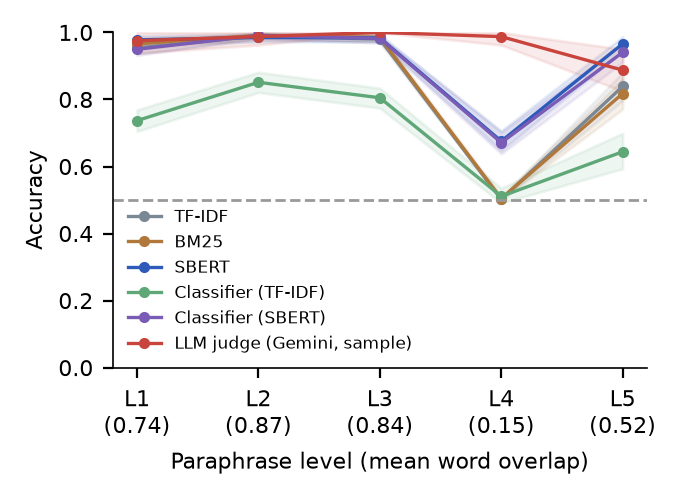
\includegraphics[width=\columnwidth]{figures/fig_degradation.png}
\caption{Accuracy per level with 95\% intervals. Local methods use the whole ladder; the LLM judge uses its 402-pair sample, hence its wider band. The dashed line marks 50\%.}
\label{fig:deg}
\end{figure}

\begin{table*}[t]
\centering\small
\begin{tabular}{@{}lccccc@{}}
\toprule
\textbf{Method} & \textbf{L1} & \textbf{L2} & \textbf{L3} & \textbf{L4} & \textbf{L5} \\
\midrule
TF-IDF & .954 (.997) & .989 (1.000) & .980 (.999) & .502 (.803) & .839 (.987) \\
BM25 & .966 (.999) & .991 (1.000) & .986 (.999) & .504 (.819) & .818 (.988) \\
SBERT & .978 (.998) & .985 (1.000) & .984 (.999) & .676 (.967) & .966 (.993) \\
Classifier (TF-IDF) & .737 (.874) & .851 (.946) & .805 (.908) & .511 (.567) & .644 (.801) \\
Classifier (SBERT) & .950 (.994) & .991 (1.000) & .982 (.999) & .671 (.916) & .941 (.984) \\
LLM judge (Gemini) & .975 & .988 & 1.000 & .988 & .887 \\
\bottomrule
\end{tabular}
\caption{Ladder accuracy, with AUC in brackets for local methods. The LLM judge has no AUC because it gives only yes or no. Intervals and recall for each label are in Appendix~\ref{app:tables}.}
\label{tab:ladder}
\end{table*}

At L1 to L3, TF-IDF, BM25, SBERT and the SBERT classifier all score about .95 or higher, so there is little to separate them (Figure~\ref{fig:deg}, Table~\ref{tab:ladder}). The TF-IDF classifier is clearly weaker throughout. L4 is where they split: TF-IDF and BM25 fall to about chance, while SBERT and the SBERT classifier reach about .67. At L5, with moderate overlap, most methods recover. This fits word overlap mattering more than the level number, but only 118 of 300 L5 rewrites survived the meaning check, so the recovery may partly reflect which rewrites were kept.

The 60 sentences kept at all levels show the same pattern at L4: TF-IDF .500, SBERT .658, SBERT classifier .717. So the L4 drop does not come from each level using different sentences.

\subsection{Why accuracy falls at L4}
\begin{figure}[t]
\centering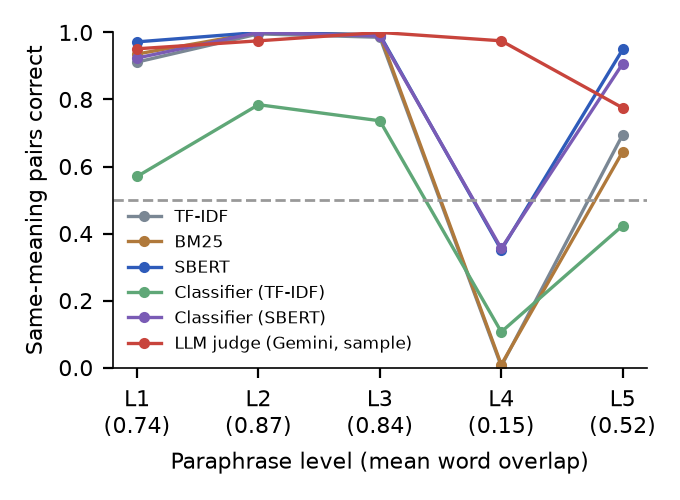
\includegraphics[width=\columnwidth]{figures/fig_recall_same.png}
\caption{Share of same-meaning pairs correctly accepted at each level.}
\label{fig:recall}
\end{figure}
At L4 almost every error is a missed paraphrase (Figure~\ref{fig:recall}). SBERT accepts only .351 of same-meaning pairs and TF-IDF only .004, while both reject all different-meaning pairs. SBERT's AUC of .967 shows it still ranks most same-meaning pairs above different-meaning ones, so its cutoff of .744 is too strict for L4. These AUC values are also helped by our fairly easy different-meaning pairs (see Limitations).

\begin{table}[t]
\centering\small
\begin{tabular}{@{}lccc@{}}
\toprule
\textbf{Method} & \textbf{Original} & \textbf{No PAWS} & \textbf{Best} \\
\midrule
TF-IDF & .502 & .502 & .764 \\
BM25 & .504 & .504 & .776 \\
SBERT & .676 & .676 & .904 \\
Classifier (TF-IDF) & .511 & .536 & .576 \\
Classifier (SBERT) & .671 & .671 & .842 \\
\bottomrule
\end{tabular}
\caption{L4 accuracy with the same scores and different cutoffs. “Best” is chosen using the answers, so it is an upper limit and not a fair score.}
\label{tab:cut}
\end{table}

The best cutoff lifts SBERT from .676 to .904 and TF-IDF from .502 to .764 (Table~\ref{tab:cut}), so the cutoff explains much of the L4 drop, and SBERT keeps a clear lead even with the best cutoff for each. We first suspected that tuning on PAWS had caused the strict cutoff, but this was wrong: removing PAWS left the cutoff unchanged for four of the five methods. The likelier reason is that one cutoff suited to pairs sharing many words cannot also suit pairs sharing almost none.

\subsection{Acceptance against word overlap}
\label{sec:overlap}
\begin{figure}[t]
\centering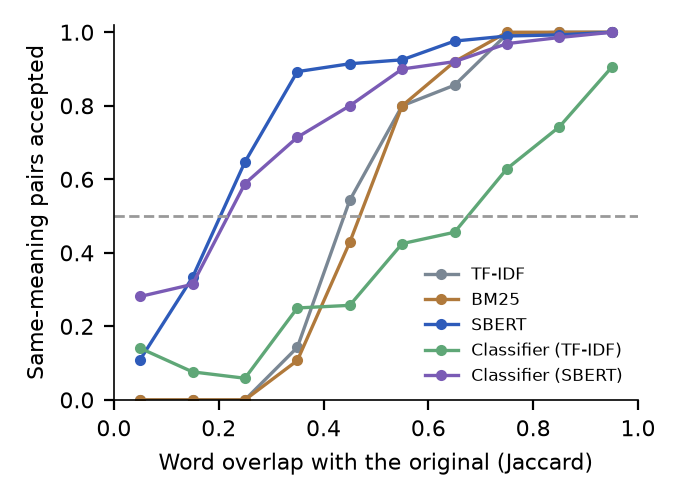
\includegraphics[width=\columnwidth]{figures/fig_overlap.png}
\caption{Same-meaning pairs accepted at each amount of word overlap, across all levels, in bins of .1. The dashed line marks 50\%.}
\label{fig:overlap}
\end{figure}
Figure~\ref{fig:overlap} sets the level number aside and groups same-meaning pairs by their overlap. TF-IDF falls below half between about .4 and .5: it accepts .14 of pairs at .3--.4, .54 at .4--.5 and .80 at .5--.6. SBERT holds on longer and falls below half between about .2 and .3: .33 at .1--.2, .65 at .2--.3 and .89 at .3--.4. These points depend on each method's cutoff. Pairs below .2 are almost all from L4, so the chart cannot fully separate overlap from the way L4 was written.

\subsection{The PAWS trick test}
\begin{figure}[t]
\centering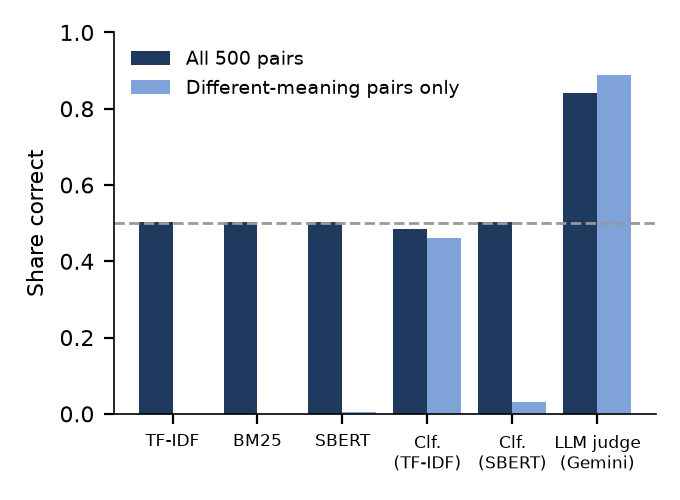
\includegraphics[width=\columnwidth]{figures/fig_paws.png}
\caption{The 500 PAWS pairs the LLM judge answered, half of each label, so chance is .50. Every method is scored on the same pairs.}
\label{fig:paws}
\end{figure}
\begin{table}[t]
\centering\small
\begin{tabular}{@{}lccc@{}}
\toprule
\textbf{Method} & \textbf{Accuracy} & \textbf{Diff. rec.} & \textbf{AUC} \\
\midrule
TF-IDF & .442 & .000 & .481 \\
BM25 & .442 & .000 & .484 \\
SBERT & .443 & .007 & .631 \\
Classifier (TF-IDF) & .507 & .478 & .521 \\
Classifier (SBERT) & .456 & .049 & .632 \\
\bottomrule
\end{tabular}
\caption{Local methods on the full PAWS test (8,000 pairs), where always answering “same” would score .442 and always answering “different” would score .558, more than any method here. “Diff. rec.” is recall on different-meaning pairs.}
\label{tab:paws}
\end{table}
TF-IDF and BM25 cannot work here, since these pairs share nearly all their words (Table~\ref{tab:paws}). SBERT also accepts almost every pair, although its AUC of .631 shows some signal. For example, it scores 1.00 for two sentences that swap the birthplace and the destination of a move between Arkansas and Tennessee, and the LLM judge correctly rejects them. The TF-IDF classifier's .507 is close to a coin flip (AUC .521), not a real gain. Its weakness is built in: a TF-IDF vector ignores word order, so two sentences that only swap words have almost identical vectors, and the features $[|u-v|, u \odot v]$ carry almost no sign of the swap.

On the sample (Figure~\ref{fig:paws}), the LLM judge scored .842 (95\% interval .808 to .872) against SBERT's .502 (.458 to .548). The intervals do not overlap. Because both methods saw the same pairs, we also ran an exact McNemar test \citep{mcnemar1947}: the LLM judge alone was right on 221 pairs and SBERT alone on 51 ($p \approx 2 \times 10^{-26}$), so the gap is clear.

\subsection{Other test sets}
\begin{table*}[t]
\centering\small
\begin{tabular}{@{}lccccc@{}}
\toprule
\textbf{Dataset} & \textbf{TF-IDF} & \textbf{BM25} & \textbf{SBERT} & \textbf{Classifier (TF-IDF)} & \textbf{Classifier (SBERT)} \\
\midrule
MRPC test (1,725) & .712 & .703 & .709 & .620 & .656 \\
QQP held-out (35,430) & .659 & .665 & .768 & .767 & .775 \\
\bottomrule
\end{tabular}
\caption{Accuracy of local methods on standard test sets.}
\label{tab:other}
\end{table*}
On QQP, SBERT, the SBERT classifier and the TF-IDF classifier score about the same (.77), ahead of TF-IDF and BM25 (Table~\ref{tab:other}). On MRPC, where pairs naturally share many words, TF-IDF does as well as SBERT, so simple methods remain reasonable when overlap is high. These scores are lower than published results for fine-tuned models, which is expected for methods with fixed features and one cutoff.

\subsection{Cost}
\begin{figure}[t]
\centering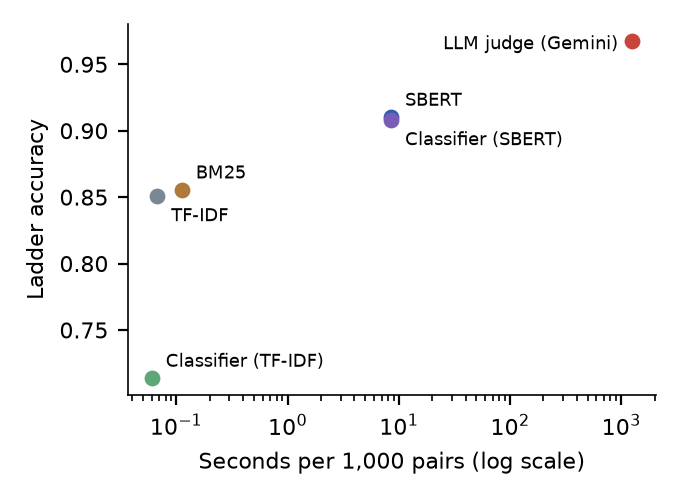
\includegraphics[width=\columnwidth]{figures/fig_cost.png}
\caption{Time against accuracy on the pairs the LLM judge answered. Time is on a log scale.}
\label{fig:cost}
\end{figure}
\begin{table}[t]
\centering\small
\begin{tabular}{@{}lcc@{}}
\toprule
\textbf{Method} & \textbf{s per 1,000} & \textbf{Accuracy} \\
\midrule
TF-IDF & 0.07 & .851 \\
BM25 & 0.11 & .856 \\
SBERT & 8.6 & .910 \\
Classifier (TF-IDF) & 0.06 & .714 \\
Classifier (SBERT) & 8.6 & .908 \\
LLM judge (Gemini) & 1,252 & .968 \\
\bottomrule
\end{tabular}
\caption{Seconds per 1,000 pairs, and accuracy on the same ladder sample.}
\label{tab:cost}
\end{table}
Local timings are the median of three runs on the same 1,000 ladder pairs on a laptop CPU (Figure~\ref{fig:cost}, Table~\ref{tab:cost}). The LLM figure uses the median call of 1.25 s, sent one at a time over the network; the mean was 4.35 s because free-tier throttling made some calls take minutes. Each call used about 74 tokens. We used the free tier, but at the listed paid price of \$0.25 per million input tokens and \$1.50 per million output tokens (checked 31 October 2026)\footnote{\url{https://ai.google.dev/gemini-api/docs/pricing}} this is about \$0.02 per 1,000 pairs. For sentences this short, the real limits are speed and the daily quota, not price. The TF-IDF classifier's slightly lower time than TF-IDF is timing noise, since it does more work. Batched local runs and single network calls are not perfectly comparable, but a gap of about 150 times over SBERT is too large to be explained by that alone.

\subsection{Human check of the labels}
\label{sec:human}
Because an LLM decided the ladder labels, one author read 150 pairs without seeing Claude's decisions: 30 per level, 114 that Claude kept and 36 that it rejected. Rejected pairs were deliberately oversampled so that both kinds of decision were tested, so the figures do not describe the whole ladder. The reader then reviewed the 32 disagreements with Claude's decisions visible and changed 20 answers. Table~\ref{tab:human} gives both results, using Cohen's kappa \citep{cohen1960} to correct agreement for chance, and Appendix~\ref{app:tables} breaks them down by level.

\begin{table}[t]
\centering\small
\begin{tabular}{@{}lcc@{}}
\toprule
\textbf{Measure} & \textbf{Blind} & \textbf{After review} \\
\midrule
Kept pairs agreed with & 112/114 & 113/114 \\
Rejected pairs agreed with & 6/36 & 25/36 \\
Reader answered “same” & 142/150 & 124/150 \\
Overall agreement & 78.7\% & 92.0\% \\
Cohen's kappa & 0.20 & 0.76 \\
\bottomrule
\end{tabular}
\caption{Agreement between the reader and Claude. Only the blind column is an independent check, since the reader had seen Claude's decisions for the review.}
\label{tab:human}
\end{table}

When blind, the reader agreed with 112 of the 114 kept pairs, so there is little sign that kept pairs had changed meaning. This is weaker evidence than it looks, because the reader accepted most pairs either way. The reader agreed with only 6 of the 36 rejections, so Claude may have over-rejected, which would remove valid hard paraphrases from the ladder and flatter accuracy. Some of the disagreements came from the reader instead: 19 of the 20 changed answers were on rejected pairs, after a closer look at changes such as “Pine Gap facility” becoming “pine Valley facilities”. The reader still judged 11 rejected pairs to keep their meaning, mostly small changes of word sense or tone such as “adult content” becoming “grownup content”. “Same meaning” clearly depends on how strictly it is applied.

\section{Failure Analysis}
Table~\ref{tab:fail} shows typical errors.

\begin{table*}[t]
\centering\small
\setlength{\tabcolsep}{4pt}
\begin{tabular}{@{}p{1.6cm}p{5.6cm}p{5.6cm}p{2.4cm}@{}}
\toprule
\textbf{Case} & \textbf{Sentence 1} & \textbf{Sentence 2} & \textbf{What went wrong} \\
\midrule
L4, same & What is the average construction salary in the UK? & How much does a typical building worker earn on average in Britain? & TF-IDF and BM25 say different \\
L1, different & Where did France focus its efforts to rebuild its empire? & When did France start in earnest to reconstruct its global empire? & SBERT says same \\
PAWS, different & Born 1841 in Lawrence County, Arkansas, Gardenhire moved with his family to Marion County, Tennessee, when he was 10 years old. & Born 1841 in Marion County, Tennessee, Gardenhire moved with his family to Lawrence County, Arkansas, when he was 10 years old. & SBERT scores 1.00; LLM correct \\
L5, same & Netflix will arrange the movie licensing from Hollywood studios, and TiVo will take care of the product technology. & Netflix will arrange a film license for a Hollywood studio, and TiVo will be in charge of product technology. & LLM says different; arguable \\
\bottomrule
\end{tabular}
\caption{Typical errors. “Same” and “different” are the labels.}
\label{tab:fail}
\end{table*}

\textbf{Local methods.} At L4 they reject valid paraphrases with few shared words, such as the salary pair in Table~\ref{tab:fail}. In the other direction, two questions about the same topic can look alike to SBERT even when they ask different things, such as “where” versus “when” France rebuilt its empire. On PAWS they accept pairs that swap who or what a sentence is about, because the words barely change.

\textbf{LLM judge.} Its one weak level is L5, with accuracy .887 and same-meaning recall .775, while it rejected every different-meaning pair. Several of its “errors” are arguable. “A film license for a Hollywood studio” is not the same as “movie licensing from Hollywood studios”, yet our review kept that pair. So part of this gap may reflect a strict judge and imperfect labels, not a clear win for SBERT at L5. On PAWS it is far from perfect: it accepted .797 of same-meaning pairs and rejected .888 of different-meaning pairs. Its mistakes include rejecting a same-meaning pair that adds “On retirement”, and accepting a pair that reorders a company name.

\section{Answers to the Research Questions}
\textbf{RQ1: Yes, with limits.} SBERT beats TF-IDF and BM25 where it matters: at L4 its accuracy is .676 against .502 and .504, with non-overlapping intervals and a much higher AUC, and at L5 it scores .966 against .839 and .818. But .676 is not graceful in absolute terms, and with its fixed cutoff SBERT still drops sharply. SBERT also gains nothing over word methods on PAWS at that cutoff.

\textbf{RQ2.} TF-IDF, BM25, SBERT and the SBERT classifier stay above 80\% at L1 to L3, fall below it at L4, and return above it at L5. The TF-IDF classifier is already below 80\% at L1, then recovers at L2 and L3 before falling again. With a 70\% threshold, the first drop is at L4 for all five local methods. The LLM judge stayed above 80\% at every level in its sample (lowest .887). Because the levels are not a staircase, overlap gives a more useful answer: with these cutoffs, TF-IDF stops accepting most paraphrases below about .4--.5 overlap and SBERT below about .2--.3 (Section~\ref{sec:overlap}).

\textbf{RQ3: Yes against our classifiers, but far more slowly.} The LLM judge scored .842 on 500 PAWS pairs, against .504 and .484 for the classifiers on the same pairs, and .988 on the L4 sample against .675 for the SBERT classifier. Its money cost at list price is small, but it took about 150 times as long as SBERT per pair, depended on a network service and hit a daily quota. Our classifiers are logistic regression on fixed sentence vectors. We did not test a fine-tuned BERT model or a cross-encoder, so this does not show that an LLM beats trained classifiers in general.

\section{Discussion}
\textbf{Overlap, not level, is what matters.} The clearest single pattern is that every local method's acceptance rises with word overlap (Figure~\ref{fig:overlap}). The ladder was designed as five steps of increasing difficulty, but its levels differ in how many words they change, and accuracy follows the words. For anyone building such a test, measuring overlap per pair is more informative than trusting the intended level.

\textbf{A score is not a decision.} SBERT's high AUC with low accuracy at L4 shows that a good similarity score can still give poor yes/no answers if one fixed cutoff is used everywhere. In practice, a cutoff tuned on data like the target use case, or a cutoff that depends on overlap, could recover much of the gap, although our best-cutoff figures are an upper limit and were chosen with the answers.

\textbf{The two failure modes need different tools.} Heavy rewording defeats word methods but not meaning vectors, while word swaps defeat both. The LLM judge was the only method that handled both in our tests. Its cost is mostly time and quota, so it fits best as a second step for the small share of pairs where a wrong answer is expensive.

\textbf{Practical recommendation.} Use SBERT as the default, as it offers the best accuracy for its speed outside adversarial data, and tune its cutoff on data resembling the real use case. Use TF-IDF or BM25 only when pairs are known to share most of their words. Send an LLM only the cases where small changes matter, such as word-swap or entity-swap pairs. A two-step system that uses SBERT first and the LLM for uncertain pairs looks sensible, but we did not test it.

\section{Conclusion}
Word-based methods work well until the words change, then fail. SBERT copes noticeably better, and much of the failure that remains comes from where its cutoff sits. Neither approach solves PAWS, where the words stay and the meaning moves. The LLM judge handled both challenges best in our sample, but it is far slower and limited by quota. Choosing a method therefore depends on what kind of difference matters in the task and how many pairs must be checked. The biggest improvement to this study would be two independent human readers with an agreed definition of “same meaning”, on more pairs, and a larger LLM sample on the ladder.

\section*{Limitations}
\textbf{The meaning check was done by an LLM.} Ladder labels rest on Claude's reading. The blind human check covered only 150 pairs with one reader, who is also an author, and agreement beyond chance was low (Section~\ref{sec:human}). An LLM judge may agree with an LLM reviewer more easily than a person would, so its ladder scores could be flattered. The PAWS result does not have this problem, as PAWS has its own labels.

\textbf{Selection effects.} Rejected rewrites were removed per level, most of all at L5 (118 of 300 kept). If Claude over-rejected, valid hard paraphrases are missing from the ladder and accuracy is flattered. Level 1 was filtered further (770 rejected candidates, 938 bans), and sentences had to allow two WordNet swaps, which favours sentences with swappable words. Some awkward Level 1 rows and AG News sentences that rely on earlier context may remain.

\textbf{Easy different-meaning pairs.} They come from different sentences (mean similarity of originals about .20), so nearly every method rejects them. Ladder results mostly test recognising paraphrases, and PAWS tests the harder direction.

\textbf{Small LLM sample.} The judge answered 402 ladder pairs (two appear twice, so these and the 500 PAWS pairs come from 900 replies), compared with 8,000 PAWS pairs and the whole ladder for local methods, and only one main model was used. An earlier run of \texttt{gemini-3.5-flash-lite} stopped at its daily limit after 486 replies. It agreed with the main model on all 78 pairs both answered, but both come from one company.

\textbf{No fine-tuned model.} Our trained classifiers use logistic regression on fixed vectors. A fine-tuned BERT model or cross-encoder may do far better on PAWS, and we did not test one.

\textbf{QQP overlap.} 27.7\% of held-out QQP pairs share a question with the training sample. We did not test whether this affects the scores.

\textbf{Self-preference test not completed.} We planned to see whether Qwen rates its own rewrites more kindly. It stopped at 316 of 999 pairs on Groq's limit of 1,000 requests a day and we dropped it, so we have no evidence on that question.

\textbf{Cutoffs and levels.} Each local method uses one cutoff for all levels, and the best-cutoff values cannot be reached in practice without knowing the answers. The levels do not form a steady ramp in word change, so “level” should not be read as a precise scale of difficulty.

\textbf{English only and short sentences.} All sentences are English and 8 to 25 words long. Longer texts, other languages and other domains may behave differently, and the LLM's cost would grow with text length.

\section*{Ethics Statement}
All datasets are public, and no personal data was collected. LLMs wrote the Level 2 to 4 paraphrases and reviewed meaning for the ladder, as described above, and their output can contain errors. A system that uses these methods to flag plagiarism or duplicates should keep a human in the loop, since our results show that each method can be confidently wrong.

\bibliography{references}
\bibliographystyle{acl_natbib}

\appendix

\section{Prompts}
\label{app:prompts}
Every Level 2 to 4 prompt ended with the same rules: “Keep exactly the same meaning: do not add, remove, or answer anything. If it is a question, keep it a question. Reply with only the rewritten sentence.” Before the rules, each level used one instruction:
\begin{itemize}\setlength{\itemsep}{2pt}\setlength{\parskip}{0pt}
\item \textbf{L2} (temperature 0.2): “Rewrite this sentence by changing only its grammatical structure: reorder clauses or phrases, or switch between active and passive voice. Keep the same words wherever possible. If no restructuring keeps the exact meaning, make only a small safe change in word order instead.”
\item \textbf{L3} (temperature 0.2): “Paraphrase this sentence with minimal changes: reword only a few words or phrases and keep most of the original wording.”
\item \textbf{L4} (temperature 0.9): “Paraphrase this sentence aggressively: use different vocabulary and a different sentence structure, reusing as few of the original words as possible (names, numbers and technical terms may stay).”
\end{itemize}
The LLM judge received: “Do these two sentences have the same meaning? Answer only yes or no.”, followed by the two sentences on separate lines. Replies starting with “yes” or “no” were accepted; none were invalid.

\section{Further Results}
\label{app:tables}
Table~\ref{tab:ci} gives the 95\% intervals for ladder accuracy and Table~\ref{tab:recall} the recall for each label. Table~\ref{tab:hclevel} breaks the human check down by level.

\begin{table*}[t]
\centering\small
\begin{tabular}{@{}lccccc@{}}
\toprule
\textbf{Method} & \textbf{L1} & \textbf{L2} & \textbf{L3} & \textbf{L4} & \textbf{L5} \\
\midrule
TF-IDF & .936--.972 & .978--.998 & .969--.991 & .500--.507 & .797--.881 \\
BM25 & .950--.982 & .983--.998 & .975--.995 & .500--.511 & .771--.860 \\
SBERT & .964--.990 & .972--.996 & .973--.993 & .647--.707 & .945--.987 \\
Classifier (TF-IDF) & .705--.769 & .821--.881 & .774--.834 & .491--.536 & .593--.699 \\
Classifier (SBERT) & .932--.968 & .983--.998 & .969--.991 & .638--.702 & .911--.966 \\
LLM judge (Gemini) & .938--1.000 & .963--1.000 & 1.000--1.000 & .963--1.000 & .825--.950 \\
\midrule
Pairs (local) & 498 & 464 & 554 & 450 & 236 \\
Pairs (LLM) & 81 & 81 & 80 & 80 & 80 \\
\bottomrule
\end{tabular}
\caption{95\% bootstrap intervals for ladder accuracy, resampling base sentences.}
\label{tab:ci}
\end{table*}

\begin{table*}[t]
\centering\small
\begin{tabular}{@{}lccccc@{}}
\toprule
\textbf{Method} & \textbf{L1} & \textbf{L2} & \textbf{L3} & \textbf{L4} & \textbf{L5} \\
\midrule
TF-IDF & .912 / .996 & .996 / .983 & .986 / .975 & .004 / 1.000 & .695 / .983 \\
BM25 & .936 / .996 & 1.000 / .983 & .993 / .978 & .009 / 1.000 & .644 / .992 \\
SBERT & .972 / .984 & 1.000 / .970 & .993 / .975 & .351 / 1.000 & .949 / .983 \\
Classifier (TF-IDF) & .570 / .904 & .784 / .918 & .736 / .874 & .107 / .916 & .424 / .864 \\
Classifier (SBERT) & .924 / .976 & 1.000 / .983 & .989 / .975 & .356 / .987 & .907 / .975 \\
LLM judge (Gemini) & .951 / 1.000 & .975 / 1.000 & 1.000 / 1.000 & .975 / 1.000 & .775 / 1.000 \\
\bottomrule
\end{tabular}
\caption{Recall on same-meaning / different-meaning pairs. Errors at L4 and L5 are almost all missed paraphrases.}
\label{tab:recall}
\end{table*}

\begin{table}[t]
\centering\small
\setlength{\tabcolsep}{4pt}
\begin{tabular}{@{}lcccc@{}}
\toprule
\textbf{Level} & \textbf{Pairs} & \textbf{Kept} & \textbf{Rejected} & \textbf{Overall} \\
\midrule
\multicolumn{5}{@{}l}{\emph{Blind}} \\
L1 & 30 & 22/22 & 0/8 & .733 \\
L2 & 30 & 21/22 & 3/8 & .800 \\
L3 & 30 & 26/26 & 0/4 & .867 \\
L4 & 30 & 22/22 & 1/8 & .767 \\
L5 & 30 & 21/22 & 2/8 & .767 \\
\textbf{All} & 150 & 112/114 & 6/36 & .787 \\
\midrule
\multicolumn{5}{@{}l}{\emph{After review}} \\
L1 & 30 & 22/22 & 4/8 & .867 \\
L2 & 30 & 21/22 & 6/8 & .900 \\
L3 & 30 & 26/26 & 3/4 & .967 \\
L4 & 30 & 22/22 & 5/8 & .900 \\
L5 & 30 & 22/22 & 7/8 & .967 \\
\textbf{All} & 150 & 113/114 & 25/36 & .920 \\
\bottomrule
\end{tabular}
\caption{Human check by level. “Kept” and “Rejected” count the pairs where the reader agreed with Claude's decision.}
\label{tab:hclevel}
\end{table}

\section{Reproducibility}
\label{app:repro}
All code, our own data and every output are in the project repository, with a README giving the run order and a notebook that recreates every table and figure from the saved outputs without API keys. All sampling uses seed 42. The classifiers use scikit-learn logistic regression ($C = 1$, up to 1,000 iterations). SBERT vectors are normalised, so their dot product is the cosine. Local experiments ran on a laptop CPU with Python 3.12; no GPU was used. The Gemini replies are saved, and the judge script resumes where it stopped. The chosen cutoffs were TF-IDF .562, BM25 .592, SBERT .744, Classifier (TF-IDF) .447, Classifier (SBERT) .300.

\end{document}
